\documentclass{article}
\usepackage{hyperref}
\usepackage{listings}
\usepackage{color}
\usepackage{xcolor}
\usepackage{geometry}
\usepackage{graphicx}
\usepackage{amsmath}
\usepackage{caption}
\usepackage{subcaption}
\usepackage[capitalise]{cleveref}
\usepackage{wrapfig}
\usepackage{amssymb}

\geometry{margin=1in}
\pdfminorversion=6

\newcommand\TODO[1]{\textcolor{red}{TODO: #1}}

\newcommand\header[2]{
    \begin{center}
        {\large
        UCSD CSE 167 Assignment #1: \\
        \vspace{0.3cm}
        \Large
        #2}
    \end{center}
}

\definecolor{dkgreen}{rgb}{0,0.6,0}
\definecolor{gray}{rgb}{0.5,0.5,0.5}
\definecolor{mauve}{rgb}{0.58,0,0.82}
\lstset{frame=tb,
        aboveskip=3mm,
        belowskip=3mm,
        showstringspaces=false,
        columns=flexible,
        basicstyle={\small\ttfamily},
        numbers=none,
        numberstyle=\tiny\color{gray},
        keywordstyle=\color{blue},
        commentstyle=\color{dkgreen},
        stringstyle=\color{mauve},
        breaklines=true,
        breakatwhitespace=true,
        tabsize=2
}

% Taken from https://tex.stackexchange.com/questions/83085/how-to-improve-listings-display-of-json-files

\colorlet{punct}{red!60!black}
\definecolor{delim}{RGB}{20,105,176}
\colorlet{numb}{magenta!60!black}

\lstdefinelanguage{json}{
    basicstyle=\normalfont\ttfamily,
    numberstyle=\scriptsize,
    stepnumber=1,
    numbersep=8pt,
    showstringspaces=false,
    breaklines=true,
    frame=lines,
    tabsize=2,
    literate=
     *{0}{{{\color{numb}0}}}{1}
      {1}{{{\color{numb}1}}}{1}
      {2}{{{\color{numb}2}}}{1}
      {3}{{{\color{numb}3}}}{1}
      {4}{{{\color{numb}4}}}{1}
      {5}{{{\color{numb}5}}}{1}
      {6}{{{\color{numb}6}}}{1}
      {7}{{{\color{numb}7}}}{1}
      {8}{{{\color{numb}8}}}{1}
      {9}{{{\color{numb}9}}}{1}
      {:}{{{\color{punct}{:}}}}{1}
      {,}{{{\color{punct}{,}}}}{1}
      {\{}{{{\color{delim}{\{}}}}{1}
      {\}}{{{\color{delim}{\}}}}}{1}
      {[}{{{\color{delim}{[}}}}{1}
      {]}{{{\color{delim}{]}}}}{1},
}

\hypersetup{colorlinks=true}


\begin{document}

\header{1}{2D Graphics}
\setcounter{section}{-1}

\begin{figure}[ht]
    \centering
    \caption{Images we will produce in this homework.}
    \label{fig:teaser}
\end{figure}

Computer graphics is the field that studies how to process \emph{visual data}, such as shapes, volumes, and lights. \textbf{Images} are an important class of visual data: they can be the pictures recorded by the camera of your cellphone or a DSLR, outputs of video games or movie visual effects, legends and arrows on Google map telling you where to go next, or visualization of the radio waves coming from a black hole. An important subfield of computer graphics, rendering, studies the generation of images.

\begin{figure}[h]
    \centering
    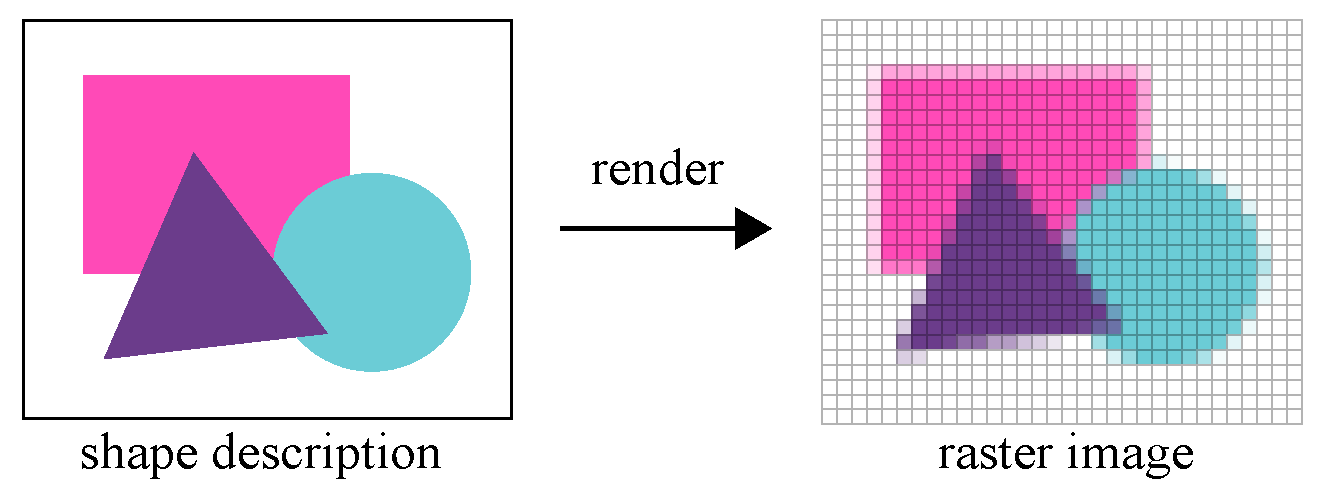
\includegraphics[width=0.6\linewidth]{imgs/render2d.pdf}
    \caption{In this homework, we will render a set of 2D shapes into a raster image.}
    \label{fig:render2d}
\end{figure}

In our first homework, we will implement a 2D renderer that takes a set of simple shapes (circle, squares, and triangles), and turn them into a raster image (\cref{fig:render2d}). A raster image is a particular kind of image that represent 2D contents using a grid of \emph{pixels}, where each pixel denotes the color at that location. Raster images are convienient because our displays (and our camera sensor) usually also represent images as a grid of pixels.

Before you start coding, we recommend you to go through the whole handout to have some ideas of what needs to be done.

\paragraph{Submission.} Submit your code and the outputs of your code through Canvas. In addition, for the quizzes below, answer them through the Gradescope (you can access it through Canvas).

\paragraph{Grading.} We will compare your outputs to our reference solutions. The points of the quizes are included in the total points on the section titles.

\paragraph{Colloboration policy.} We expect you to write the code on your own. Feel free to discuss between the peers and ask us questions though!

\section{Building Balboa}

We are going to build our code on top of a currently barebone codebase \emph{balboa}. Balboa already includes all the third party libraries (stb\_image and stb\_image\_write) in its repository.
All you need to do is to clone the repo and build it using CMake (assuming you are in a Unix-like system):
\begin{lstlisting}[language=bash]
  git clone https://github.com/BachiLi/balboa_public
  mkdir build
  cd build
  cmake ..
  make -j
\end{lstlisting}

After building, you should see an executable \lstinline{balboa}. Try typing the following command:
\begin{lstlisting}[language=bash]
  ./torrey -hw 1_1
\end{lstlisting}
It will generate an image \lstinline{hw_1_1.png} that is completely white.

We recommend you to quickly read through \lstinline{main.cpp} and \lstinline{hw1.cpp} to understand the structure of the code.

\section{Rendering a single circle (10 pts)}

\begin{figure}[h]
    \centering
    \begin{subfigure}[t]{0.4\linewidth}
        \centering
        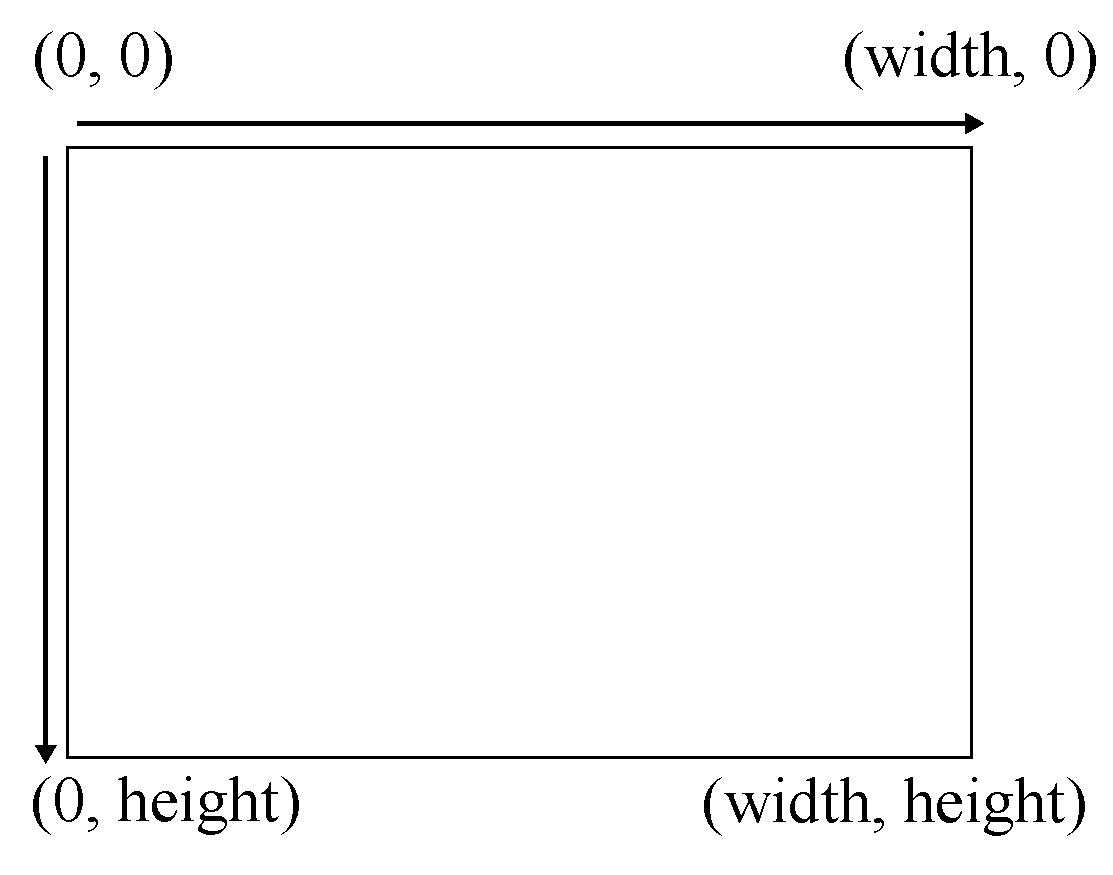
\includegraphics[width=\linewidth]{imgs/canvas.pdf}
        \caption{\label{fig:canvas}}
    \end{subfigure}
    \begin{subfigure}[t]{0.4\linewidth}
        \centering
        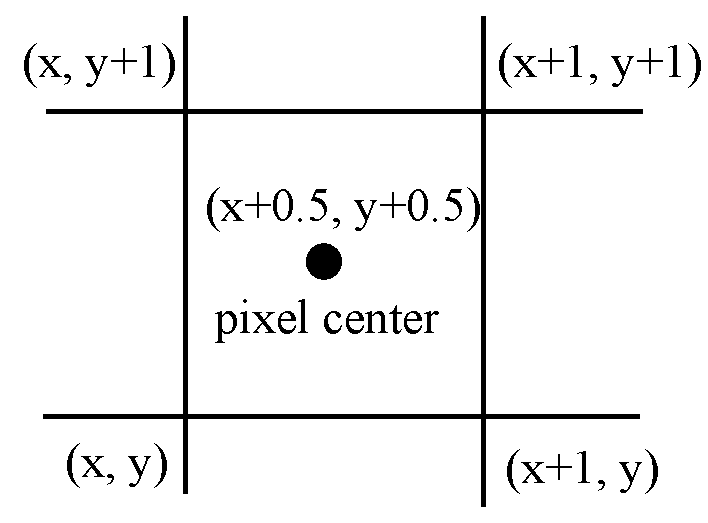
\includegraphics[width=\linewidth]{imgs/pixel.pdf}
        \caption{\label{fig:pixel}}
    \end{subfigure}
    \caption{(a) The coordinate system of the ``canvas'' we will draw our shapes on. (b) The pixel center of for pixel $(x, y)$ locates at $(x+0.5, y+0.5)$.}
\end{figure}

In the first part of this homework, we will render a single circle on our image. We are given a white ``canvas'' (\cref{fig:canvas}), where in this part we assume it to be of size $640 \times 480$. We need a \textbf{coordinate system} to talk about points on this canvas. The usualy convention for an image is that the top left is the origin, and the x-axis points towards right, and the y-axis points downwards. We are futher given the center, radius, and color of the circle. These are command line arguments that we will parse for you.

To render an image, we need to determine the color for each pixel. For this part, we focus on determining the color of the center of the pixel (\cref{fig:pixel}). To determine the pixel color, we decide whether the pixel center hits the circle or not. If it hits the circle, then we decide that the pixel's color is the circle's color. Otherwise, we decide that the pixel's color is the background color (by default, let's say it's $(1, 1, 1)$). How to decide whether the pixel center hits the circle? That's for you to figure out!

Balboa provides a few utitilies that will be useful for this homework: \lstinline{Vector2}, \lstinline{Vector3}, and \lstinline{Image3}. They are defined in \lstinline{vector.h} and \lstinline{image.h}. 

\paragraph{Vectors.} \lstinline{Vector2} and \lstinline{Vector3} are utilities for representing 2D and 3D vectors. You can access their members using \lstinline{.x}, \lstinline{.y}, and \lstinline{.z}. We overloaded a few common operators so that you can add and subtract vectors, and multiply them with scalars:
\begin{lstlisting}[language=C++]
Vector2 v0 = ..., v1 = ...;
v0 + v1; // vector addition
v0 - v1; // subtraction
v0 * Real(0.5) // multiply by a scalar
v0 / Real(0.5) // divide by a scalar
dot(v0, v1) // dot product between the two vectors
normalize(v0) // returns a vector with same direction as v0, but with magnitude of 1
\end{lstlisting}
In balboa, we represent floating point numbers using the type \lstinline{Real}. It is by default defined to be a \lstinline{double}. It is designed such that when you want to switch to single precision float (maybe for less memory cost), you can switch a single line in \lstinline{balboa.h}.
\begin{lstlisting}[language=C++]
using Real = double;
\end{lstlisting}

\begin{figure}[h]
    \centering
    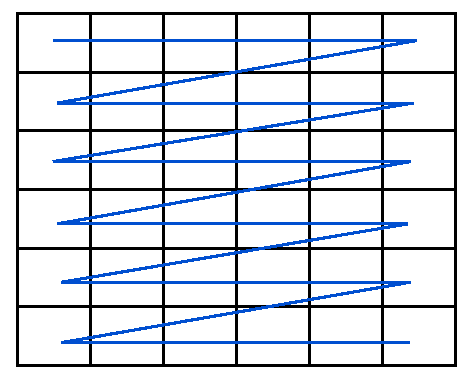
\includegraphics[width=0.4\linewidth]{imgs/scanline.pdf}
    \caption{Storing a 2D image in an 1D array by scanning the image.}
    \label{fig:scanline}
\end{figure}

\paragraph{Images.} \lstinline{Image3} represents a 3-channel raster image (usually storing red, green, blue value at each channel respectively). We store the 2D image in a 1D array using a scanline (\cref{fig:scanline}). You can access the 2D image using the \lstinline{()} operator:
\begin{lstlisting}[language=C++]
Image3 img(640 /* width */, 480 /* height */);
Vector3 val = img(50, 20); // reading values from location (50, 20)
img(30, 60) = Vector3{0.5, 0.6, 0.7}; // writing values to location (30, 60)
img.width; // 640
img.height; // 480
imwrite("image.png", img); // write the image to the disk
Image3 img2 = imread3("image2.png"); // read an image from the disk
\end{lstlisting}
The pixel values are stored as \lstinline{Real} in the memory. When we write the image into a file, the file format can often only supports 8-bit integers. The conversion is made in the \lstinline{imwrite} function, where we apply a \href{https://en.wikipedia.org/wiki/Gamma_correction}{gamma correction} to encode the image (with $\gamma=\frac{1}{2.2}$). We will likely talk about gamma correction in the class.

You should be ready to implement the circle rendering code at this point. 
To see your results, in terminal, type:
\begin{lstlisting}[language=bash]
  ./balboa -hw 1_1 -center 200 300 -radius 100 -color 0.3 0.7 0.5
  ./balboa -hw 1_1 -center -50 250 -radius 100 -color 0.7 0.3 0.3
  ./balboa -hw 1_1 -center 600 250 -radius 150 -color 0.3 0.5 0.7
  ./balboa -hw 1_1 -center 250 470 -radius 50 -color 0.7 0.5 0.7
\end{lstlisting}
or just any parameter you like! \cref{fig:hw1_1} shows our rendering for the first command.

\begin{figure}[ht]
    \centering
    \includegraphics[width=0.5\linewidth]{imgs/hw_1_1.png}
    \caption{References for Homework 1.1.}
    \label{fig:hw1_1}
\end{figure}

If you see your circles, congratulations! If you have not done graphics-related stuff before, this is likely the first time you have use code to generate an image from scratch. This is what makes computer graphics fun at least for me: you paint on a canvas using code (and sometimes math) instead of a brush. This makes people who are not that good in traditional art capable of generating beautiful pictures (yes, the images you generate will become prettier from now on). Furthermore, unlike things like Stable Diffusion, you maintain full control of the process: at this point, you know exactly how each pixel is generated, and if you don't like it, it's very easy to fix if you know how computer graphics works.

%\bibliographystyle{plain}
%\bibliography{refs}

\end{document}
